\documentclass[12pt]{paper}

\usepackage{Schwieg}
\usepackage[margin=1in]{geometry}
\usepackage{tikz}
\usepackage{verbatim}
\title{Price Theory I: Problem Set 3 Question 1}
\author{Samuel Barker\and Timothy Schwieg\and Rafeh Qureshi\and Daniel Noriega}
\begin{document}
\maketitle

\section{Setup}
We are imagining a business where an owner is looking to hire a
manager, and can select between a relative and a more talented
contractor (sub-scripted by ``R'' and ``C'' respectively). He will offer
a portion of the reported profits to the manager when he makes a job
offer. He will keep $\beta \in (0,1)$ of the reported profits and the
manager will get the rest, $(1-\beta)$. The true profits are $u+T$ where
$T$ is the talent of the manager and profits are increasing in $T$. A
twist on this is that the manager is able to steal from the profits
before it is split, but he faces a cost of stealing per dollar:
$\gamma \in (0,1)$. Additionally, there is an altruistic relationship between
the owner and the relative--this means that one of the two counts the
other's utility as his own (preferring his own utility more, of
course). There are a couple of cases that we can imagine.

Before beginning the model, however, we shall adjust some notation to
make things simpler. From here on out $(T_C+u)$ is normalized to
one. And therefore, $(T_R+u)=1-L$, where $L=T_R-T_C$, the difference
between the contractor's talent and the relative's talent.

An important fact is that we assume that both managers have outside
options. We suppose that they are both capable of achieving a wage of
$W_R$--their reservation wage--even if they are not hired.
\\

\section{Model}
First consider an \textbf{altruistic relative}--we will call this case one.
In this scenario, we can model the utility functions of the actors as follows:\\
The owner's
\begin{align*}
u_O=&~\beta(1-e_C)\\
\text{or}\\
u_O=&~\beta(1-e_R-L)
\end{align*}
where $e_i\in (0,1)$ is the amount of money the manager steals and $i$ is either the relative or contractor.\\
The contractor:
\begin{align*}
u_C=&~(1-\beta)(1-e_C)+e_C-\gamma e_C\\
u_C=&~(1-\beta)+e_C(\beta-\gamma).
\end{align*}
And finally, the altruistic son:
\begin{align*}
u_R=&~\alpha[(1-\beta)(1-L-e_R)+e_R-\gamma e_R]+(1-\alpha)[\beta(1-e_R-L)]\\
u_R=&~\alpha[(1-\beta)(1-L)+e_R(\beta-\gamma)]+(1-\alpha)[\beta(1-e_R-L)].
\end{align*}
Importantly, the relative leans toward being selfish, which means that $\alpha \in (.5,1)$.

If it is the \textbf{owner who is altruistic}, we can quickly see how these change the model--we will call this case two. The utility of the owner becomes:
\begin{align*}
u_O=&~\alpha[\beta(1-e_R-L)]+(1-\alpha)[(1-\beta)(1-L)+e_R(\beta-\gamma)]\\
or\\
u_O=&~\alpha[\beta(1-e_C)]+(1-\alpha)W_R
\end{align*}
where the first equation shows the owner's utility if his relative is working for him, and the latter shows his relative making his reservation wage.

In this scenario, the relative's utility would simply be:
\begin{align*}
u_R=&~(1-\beta)(1-L)+e_R(\beta-\gamma).
\end{align*}

And lastly, it is obvious that the utility of the contractor is unchanged--this guy is never altruistic.


\section{Part A}
If we take a look again at the utilities of the managers, we can
immediately see when they will, and when they won't steal. First,
check when the owner is not altruistic--which is case 1.
\subsection{Case 1}
Due to this, for the non-altruistic people, their utility is
equivalent to their profit: $\Pi_i$ where $i\in \{C,R,O\}$. Consider the
owner's profit: in this case, he is only interested in his own
profit. And since the contractor can always provide a higher amount of
profit to the owner (he is more talented, whereas the relative is
maybe a little slow), using a Bertrand argument, we can see that the
relative will never steal since the contractor can always offer a
better deal. If the relative doesn't steal, and contractor steals the
amount of the difference in talent, then the owner should be
indifferent between them. Thus, to make things simple (rather than
assuming the contractor steals some increasingly small $\epsilon$ less than
the difference in talent, which is boring), we will assume that the
owner likes the spunk of the thief and rewards him with a job.
\begin{align*}
\Pi_C=&~(1-\beta)+e_C(\beta-\gamma)
\end{align*}
and the partial with respect to $e_C$
\begin{align*}
\frac{\partial \Pi_C}{\partial e_C}=&~\beta-\gamma
\end{align*}
\textbf{Thus, when $\beta>\gamma$ he will steal.} He will steal until the
owner's profit is the same as it would have been with the relative of
dubious talent (i.e. $e_C=L=T_C-T_R$). He will continue to steal that
exact same amount, until reaching a $\tilde{\beta}$, which is a
$\beta$ so large that he makes the same as he would with his outside
options--mathematically, we mean:
\begin{align*}
\Pi_C=&~(1-\tilde{\beta})+L(\tilde{\beta}-\gamma)=W_R
\end{align*}
After that point, he must steal more than $L$ to maintain at least
$\Pi_C=W_R$. We can see this easily in graphical form. Consider
\textbf{Figure 1}.

\begin{figure}[h!]
  \centering
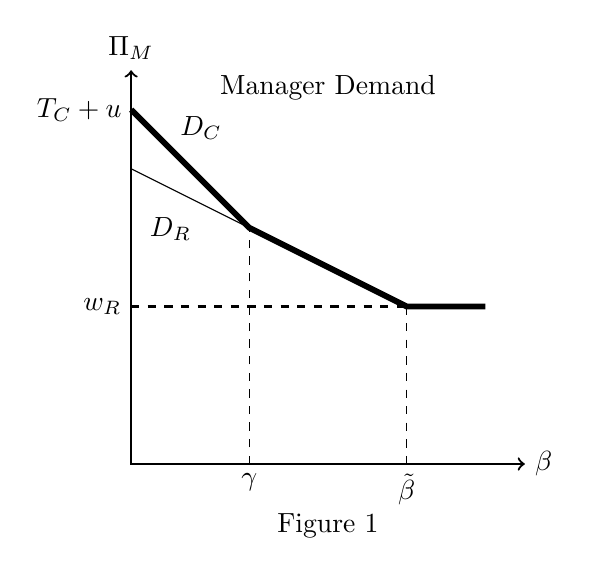
\begin{tikzpicture}[scale=0.5]

\draw[thick,<->] (0,10) node[above]{$\Pi_{M}$}--(0,0)--(10,0) node[right]{$\beta$};

\node [left] at (0,9) {$T_C + u$};
\node [left] at (0,4){ $w_R$};

\node [below] at (7,0) {$\tilde{\beta}$};
\node [below] at (3,0) {$\gamma$};
\node [above right] at (1,8){$D_C$};
\node [above] at (5,9){Manager Demand};

\draw[line width=.75mm](0,9)--(3,6)--(7,4)--(9,4);
\draw (0,7.5)--(3,6);
\node [below] at (1,6.5){$D_R$};

\draw[dashed](7,4)--(7,0);
\draw[dashed](3,0)--(3,6);
\draw[dashed, line width=.5mm](0,4)--(9,4);

\node[below] at (5,-1){Figure 1};

\end{tikzpicture}
\end{figure}

There we can easily track the story from left to right: the contractor doesn't steal until the shares of the owner that he would get from stealing outweigh the costs--when $\gamma=\beta$, and then steals at $e_C=L$ until $\tilde{\beta}$ at which he has to increase the amounts he steals to compensate himself up to his outside option, namely $W_R$.

Because we are interested in when the owner can keep people from stealing profits, we need to see this story from the owner's perspective. \textbf{Since the owner chooses $\beta$, under what conditions would he choose $\beta \leq \gamma$ thus causing the manager to not hide profits?} To answer this, consider \textbf{Figure 2} and \textbf{Figure 3}.

There is a simple condition in which you get the result in Figure 2 instead of the result in Figure 3. Namely, that condition is when:
\begin{align*}
(1-L)(\gamma-\tilde{\beta})&> \gamma L\\
\implies 1+\frac{\tilde{\beta}(L-1)}{\gamma} &>2L
\end{align*}
Intuitively, this is a question about if, when there is theft, a larger share for the owner will be enough to compensate him for the theft while keeping the manager's profit at or above his reservation wage. Thus, in Figure 2 the owner would always maximize his profit by choosing $\beta^*=\tilde{\beta}$. Naturally, if the inequality is flipped, then we would get Figure 3. When they are equal, there would be two potential equally attractive choices.

\begin{figure}[h!]
  \centering
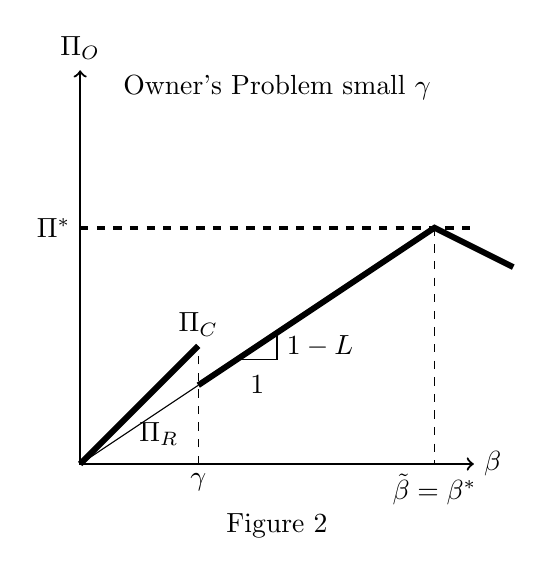
\begin{tikzpicture}[scale=0.5]

\draw[thick,<->] (0,10) node[above]{$\Pi_{O}$}--(0,0)--(10,0) node[right]{$\beta$};

\node [left] at (0,6) {$\Pi^{*}$};

\node [below] at (9,0) {$\tilde{\beta} = \beta^{*}$};
\node [below] at (3,0) {$\gamma$};

% \node [above] at (5,10){};
\node [above] at (5,9){Owner's Problem small $\gamma$};

\draw[line width=.75mm](0,0)--(3,3);
\draw[line width=.75mm](3,2)--(9,6)--(11,5);
\draw (0,0)--(3,2);

\node [above] at (3,3){$\Pi_C$};
\node [below] at (2,1.3){$\Pi_R$};

\draw (4,2.66)--(5,2.66)--(5,3.33);
\node [below] at (4.5,2.5){$1$};
\node [right] at (5,3){$1-L$};

\draw[dashed](9,6)--(9,0);
\draw[dashed](3,0)--(3,3);
\draw[dashed, line width=.5mm](0,6)--(10,6);

\node[below] at (5,-1){Figure 2};

\end{tikzpicture}
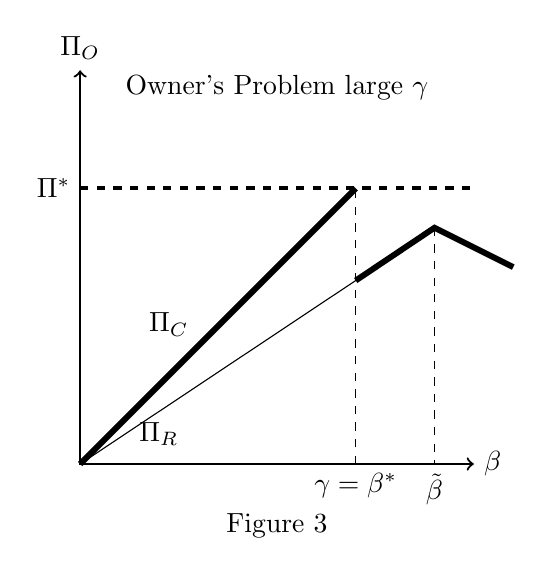
\begin{tikzpicture}[scale=0.5]
  \draw[thick,<->] (0,10) node[above]{$\Pi_{O}$}--(0,0)--(10,0) node[right]{$\beta$};
  \node [left] at (0,7) {$\Pi^{*}$};

\node [below] at (9,0) {$\tilde{\beta}$};
\node [below] at (7,0) {$\gamma = \beta^{*}$};

\node [above] at (5,9){Owner's Problem large $\gamma$};
%\node [above] at (5,10){};

\draw[line width=.75mm](0,0)--(7,7);
\draw[line width=.75mm](7,4.66)--(9,6)--(11,5);
\draw (0,0)--(7,4.66);

\node [above left] at (3,3){$\Pi_C$};
\node [below] at (2,1.3){$\Pi_R$};

\draw[dashed](9,6)--(9,0);
\draw[dashed](7,0)--(7,7);
\draw[dashed, line width=.5mm](0,7)--(10,7);

\node[below] at (5,-1){Figure 3};
  
\end{tikzpicture}
\end{figure}
Clearly, however, when we get the result in Figure 3, the owner could--and would--keep the manager from stealing because he would maximize his own profits by selecting $\beta=\gamma$. Therefore, the condition in which the owner can keep the manager from stealing is when $L$, $\gamma$, and $\tilde{\beta}$ are such that
\begin{align*}
1+\frac{\tilde{\beta}(L-1)}{\gamma} &>2L.
\end{align*}
\\

\subsection{Case 2} There is a second case however. Namely, when the owner is altruistic and the relative is not. There is again a similar condition for when the owner is able to keep his manager from stealing. There is an obvious one: $\gamma > \tilde{\beta}$, which would just mean that the cost of stealing was so high, it would never occur until after the reservation wage was past. Because this is a trivial solution, we will assume that $\gamma < \tilde{\beta}$.

Even with this assumption, there are two cases that are possible. To begin to see this, realize that because the owner is altruistic, for any $\beta$ small enough he will always hire his relative--because he actually gets some utility from it. We will have the relative stealing once $\beta>\gamma$, just like the contractor. And he will steal down to the amount that the owner will be indifferent between them again (recall that our owner likes some moxie, and thus will always choose the thief all else equal). Unfortunately for our burgling relative, the talented contractor will become able to do more for the owner once his line intersects the relative's. This is demonstrated below in Figures 4 and 5--the lines intersect at $\eta$. At this point, the relative couldn't outperform the contractor even if he didn't steal. However, if $\eta<\tilde{\beta}$, then our question about how the owner could keep the manager from stealing would be moot--he couldn't ever do it because the contractor would always steal the difference. Thus, only in a very particular scenario in Figure 5 will we see the owner able to keep people from stealing.

The intuition behind the argument is the same as for the previous case. Can the owner make his share large enough to compensate for the fall in profit before raising his $\beta$ to $\tilde{\beta}$? Our condition for no theft mathematically is a bit messy:

\begin{align*}
\tilde{\beta}-\gamma&>\Pi_{OR}-\Pi_{OC}\\
\Pi_{OR}&=\alpha \gamma(1-L)+(1-\alpha)(1-L)\\
\Pi_{OC}&=\alpha-(1-\alpha)W_R=\alpha-(1-\alpha)(1-\tilde{\beta})\\
\implies \tilde{\beta}-\gamma&>\alpha \gamma(1-L)+(1-\alpha)(1-L)-\alpha-(1-\alpha)(1-\tilde{\beta})
\end{align*}

Unfortunately, there isn't a convenient way of simplifying this. $\Pi_{OR}$ is the profit of the owner if he hires the relative at $\beta=\gamma$ and the relative chooses not to steal. The $\Pi_{OC}$ is the profit the owner gets from hiring the contractor at $\beta=\gamma$. Now, we argue that he is in fact hiring the relative here, but since he is actually indifferent between them at this point, it is equivalent, and easier to view it this way. Note that the owner still gets utility from the fact that the relative would make a reservation wage. If the inequality were flipped, then we know we would get theft.

\begin{figure}[h!]
  \centering
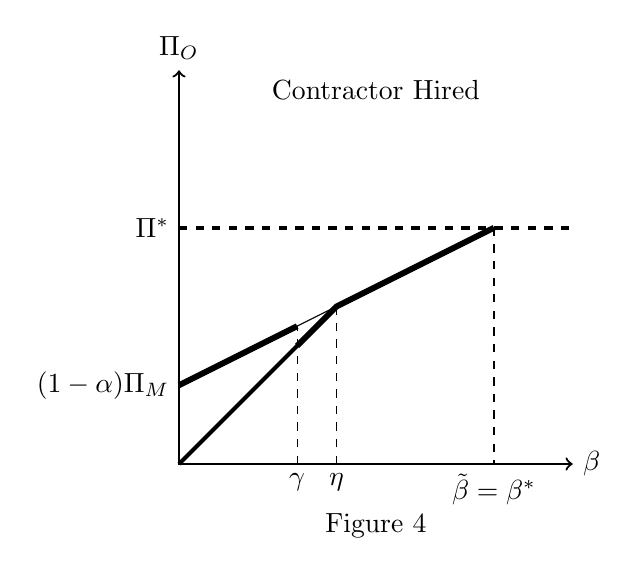
\begin{tikzpicture}[scale=0.5]

\draw[thick,<->] (0,10) node[above]{$\Pi_{O}$}--(0,0)--(10,0) node[right]{$\beta$};

\node [left] at (0,6) {$\Pi^{*}$};

\node [below] at (8,0) {$\tilde{\beta} = \beta^{*}$};
\node [below] at (3,0) {$\gamma$};
\node [below] at (4,0) {$\eta$};
\node [left] at (0,2){ $(1-\alpha) \Pi_M$};

% \node [above] at (5,10){};
\node [above] at (5,9){Contractor Hired};

\draw[line width=.5mm](0,0)--(4,4);
\draw[line width=.75mm](0,2)--(3,3.5);
\draw (3,3.5)--(4,4);
\draw[line width=.75mm](3,3)--(4,4)--(8,6);
%\draw (0,0)--(9,6);

%\node [above] at (3,3){$\Pi_C$};
%\node [below] at (2,1.3){$\Pi_R$};

\draw[dashed](8,6)--(8,0);
\draw[dashed](3,0)--(3,3.5);
\draw[dashed](4,0)--(4,4);
\draw[dashed, line width=.5mm](0,6)--(10,6);
\node[below] at (5,-1){Figure 4};
\end{tikzpicture}
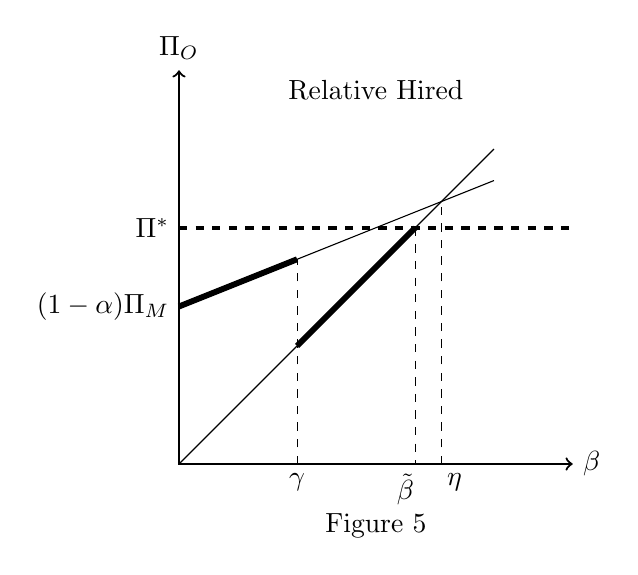
\begin{tikzpicture}[scale=0.5]

\draw[thick,<->] (0,10) node[above]{$\Pi_{O}$}--(0,0)--(10,0) node[right]{$\beta$};

\node [left] at (0,6) {$\Pi^{*}$};

\node [below] at (5.75,0) {$\tilde{\beta}$};
\node [below] at (3,0) {$\gamma$};
\node [below] at (7,0) {$\eta$};
\node [left] at (0,4){ $(1-\alpha) \Pi_M$};

% \node [above] at (5,10){};
\node [above] at (5,9){Relative Hired};

\draw(0,0)--(3,3);
\draw[line width=.75mm](0,4)--(3,5.2);%--(5,6);
\draw (3,5.2)--(5,6)--(8,7.2);
\draw[line width=.75mm](3,3)--(6,6);%--(8,6);
\draw (6,6)--(8,8);

%\node [above] at (3,3){$\Pi_C$};
%\node [below] at (2,1.3){$\Pi_R$};

\draw[dashed](6,6)--(6,0);
\draw[dashed](3,0)--(3,5.2);
\draw[dashed](6.66,0)--(6.66,6.66);
\draw[dashed, line width=.5mm](0,6)--(10,6);
\node[below] at (5,-1){Figure 5};
\end{tikzpicture}
\end{figure}

\section{Part B}
From here one out, we will assume that the owner cannot keep his managers from stealing. This implies that for a non-altruistic owner:
\begin{align}
1+\frac{\tilde{\beta}(L-1)}{\gamma} &>2L.
\end{align}
And for an altruistic owner:
\begin{align*}
\tilde{\beta}-\gamma&>\Pi_{OR}-\Pi_{OC}
\end{align*}
or, if we plug in for the profits,
\begin{align}
\tilde{\beta}-\gamma&>\alpha \gamma(1-L)+(1-\alpha)(1-L)-\alpha-(1-\alpha)(1-\tilde{\beta}).
\end{align}

Given these conditions, do we expect the owner's son to hide profits? This depends on multiple factors. First, if the owner is not the altruistic one (Case 1), then the son would never be hired (the guy just isn't talented enough). So he could not steal.

In Case 2, where the owner is altruistic, the son would steal if he was hired. This would depend, as it did above, on where $\eta$ is. Again, consider Figures 4 and 5. In Figure 4, for $\beta s$ greater than $\eta$, the contractor is able to offer enough additional profit to make up for the fact that the owner is altruistic and is thus hired. Figure 5 shows the opposite, and in this case the relative would steal from his altruistic father.

\section{Part C}
The above conclusions hold for the relative being a son-in-law who has an altruistic relationship with his wife. We could imagine the owner having an altruistic relationship with his daughter, and therefore there is indirect altruism for his son-in-law (or the other way around). However, this is effectively just choosing a different parameter for altruism. Meaning, $\alpha$ would just be multiplied through by another parameter, but the results wouldn't depend on those--the actual values of the realizations may be different, but the analysis is identical.

\section{Part D}




















\begin{comment}
\section{Model}

Consider a world where $T,u$ are observed by all, and during the
hiring process, a potential manager (either relative or contractor)
suggests a function that gives profits as a function of wages. The
owner observes this, and after seeing the other manager's offer, hires
a worker at a given wage level. Note that the profits given are the
profits that are split between the manager and the owner (after
stealing has occurred.) When there is a tie between the two managers,
this tie is always resolved by the job given to the manager that is
stealing more. The owner believes that they have spunk and respects
them for it.

Clearly the owner will accept the one that gives him the higher
payoff.  From this structure we can see that it will not be optimal
for the related manager, who is less productive, to ever steal. 
When altruism is added to the manager's package the same idea
occurs. Consider first the case where the relative is altruistic, but
still prefers himself. Let $AM$ denote the altruistic manager.

\begin{align*}
  \Pi_{AM} = \alpha \left[ (1-\beta)(1-L) + e(\beta-\gamma) \right] + (1-\alpha)\left[ \beta(1-L-e)
  \right]\\
  \deriv{\Pi_{AM}}{\beta} = (L+e-1)(2\alpha-1) < 0
\end{align*}
where $L+e-1$ is negative since it is $e - (1-L)$ which is the
negative of the reported profit in the contract of related
manager. Note that $2\alpha-1$ is positive as $\alpha \in (\frac{1}{2},1)$.

This means that he still always prefers being paid more money from the
owner, but at less of a degree. There is still no equilibrium where he
steals from the owner, as the owner only values his profits, and the
same Bertrand-Style argument above applies. In any of these
equilibria, the related manager does not receive the job, and thus him
being altruistic does not change the problem at all.

\begin{figure}
  \centering
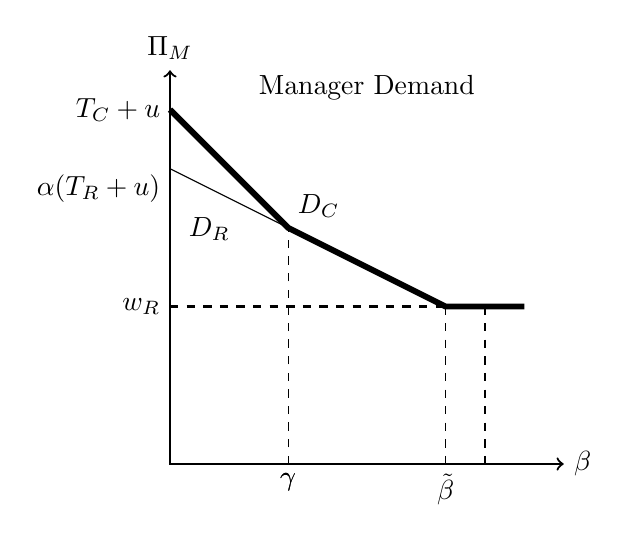
\begin{tikzpicture}[scale=0.5]

\draw[thick,<->] (0,10) node[above]{$\Pi_{M}$}--(0,0)--(10,0) node[right]{$\beta$};

\node [left] at (0,9) {$T_C + u$};
\node [left] at (0,4){ $w_R$};

\node [below] at (7,0) {$\tilde{\beta}$};
\node [below] at (3,0) {$\gamma$};
\node [above right] at (3,6){$D_C$};
\node [above] at (5,9){Manager Demand};

\draw[line width=.75mm](0,9)--(3,6)--(7,4)--(9,4);
\draw (0,7.5)--(3,6);
\node [below] at (1,6.5){$D_R$};

\draw[dashed](7,4)--(7,0);
\draw[dashed](3,0)--(3,6);
\draw[dashed, line width=.5mm](0,4)--(9,4);

\node [left] at (0,7) {$\alpha (T_R + u)$};

\draw[dashed](8,4)--(8,0);
\node [below] at (3,0) {$\gamma$};

\end{tikzpicture}
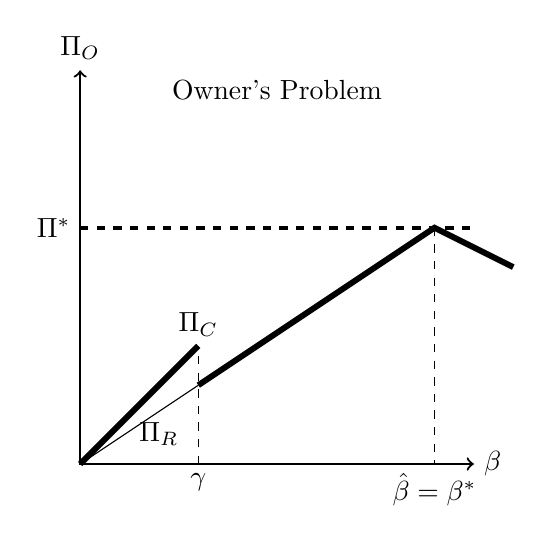
\begin{tikzpicture}[scale=0.5]

\draw[thick,<->] (0,10) node[above]{$\Pi_{O}$}--(0,0)--(10,0) node[right]{$\beta$};

\node [left] at (0,6) {$\Pi^{*}$};

\node [below] at (9,0) {$\hat{\beta} = \beta^{*}$};
\node [below] at (3,0) {$\gamma$};

% \node [above] at (5,10){};
\node [above] at (5,9){Owner's Problem};

\draw[line width=.75mm](0,0)--(3,3);
\draw[line width=.75mm](3,2)--(9,6)--(11,5);
\draw (0,0)--(3,2);

\node [above] at (3,3){$\Pi_C$};
\node [below] at (2,1.3){$\Pi_R$};

\draw[dashed](9,6)--(9,0);
\draw[dashed](3,0)--(3,3);
\draw[dashed, line width=.5mm](0,6)--(10,6);

\end{tikzpicture}
\end{figure}



When the owner is altruistic, the story changes slightly. The owner
now values the well-being of his relative, and values his profit
less. However when considering the contractor's offer, he values only
his profit. The owner will require a higher profit of the contractor
to be indifferent, as long as the relative is making less profit than
he is, and a lower profit when his relative is making more than the
owner. This means that there are equilibria where the son will steal
from his altruistic dad.


When $\beta < \gamma$ neither party wishes to steal. For some values of $\beta$ the
manager will always prefer to hire his son. The utility that is
provided by the son working is positive when $\beta = 0$ and zero for the
contractor. However the slope of the line is smaller than one.

\begin{equation*}
  \deriv{\Pi_{AO}}{\beta} = (1-L)(2\alpha-1) < 1-L < 1
\end{equation*}

It is ambiguous whether or not this line intersects the profit line of
the contractor before $\beta = \gamma$. If it intersects before, then the
manager will hire the contractor after that level of $\beta$. After $\beta =
\gamma$, the contractor will steal down to the utility produced by the
relative manager working, and the relative will not steal by the above
Bertrand Argument. This will continue to the point where the
relative's demand profit equals the reservation wage, occurring at
$\tilde{\beta}$. 

Another case is when the intersection occurs after $\beta = \gamma$. For some
$\beta > \gamma$, the relative provides higher utility than the contractor to
the owner. The relative can then steal down until the owner is at the
utility level of the contractor. The contractor is unable to steal by
the preceding Betrand argument. Let $\eta$ be the intersection between
the utility for the relative, and the profit from the contractor. If
$\tilde{\beta} < \eta$, then the relative will be hired while stealing from
the owner. If $ \tilde{\beta} > \eta$ then the contractor will be hired while
stealing. When they are equal, neither will steal and the owner will
be indifferent between hiring either. 

This means that it does matter whether or not it is the owner or the
son who is altruistic. When the owner is altruistic, he is willing to
hire his relative under certain conditions. However when the relative
is the altruistic one, he is never hired. 




 Because. Now, allow for there to be two different values of $\gamma$. The relative
has a higher value of $\gamma$. Note that since the family is not
altruistic, the manager can give the owner higher utility than the
relative can. This prevents the relative from ever stealing, due to
the Betrand argument that has prevented the lower productive member
from stealing before. Therefore increasing the area where the relative
finds it costly to steal has no binding affect on this model. The
relative does not choose to steal, so preventing him from stealing has
no affect on the outcomes.
\end{comment}






If we say that the relative is not altruistic, but instead feels guilt about stealing (modeled as higher $\gamma$), does the answer to Part B change? In short, no because Part B asks us to restricted our analysis to cases where the owner's optimal choice includes theft (i.e. the relations in equations (1) and (2) are satisfied).

Consider Case 1 where the owner is not altruistic. Since we found that the relative would never steal in this case, changing the cost of stealing for him would have no effect at all.

In Case 2, we have the same result. Because our analysis is restricted, the only item of consequence is what $\eta$ is, and that will not depend on $\gamma$. 

Of course, if we drop our restriction, then we may get different results. In fact, the restrictions are less likely to hold for large $\gamma$s. This is obvious from the equations:
\begin{align*}
1+\frac{\tilde{\beta}(L-1)}{\gamma} &>2L,
\end{align*}
and, for an altruistic owner:
\begin{align*}
\tilde{\beta}-\gamma&>\alpha \gamma(1-L)+(1-\alpha)(1-L)-\alpha-(1-\alpha)(1-\tilde{\beta})\\
&\implies\\
\tilde{\beta}+\gamma(L-1-\alpha)&>(1-\alpha)(1-L)-\alpha-(1-\alpha)(1-\tilde{\beta}).
\end{align*}
It is immediately clear that the left hand side of these equations decrease in $\gamma$, and are therefore less likely to hold for large $\gamma$s. Thus, if we allow these conditions to slip, then we may begin to get results where there is no theft (which is explored more in Part F).

\section{Part E}

The owner prefers to hire his less talented son only when he is
altruistic. When the owner is altruistic, and sufficiently so such
that the intersection between the utility of the owner and the profit
of the contractor occurs after $\tilde{\beta}$, he chooses to hire his
son.

\section{Part F}
If we think about social institutions that encourage honesty, it is natural to view this as a higher $\gamma$ level for everyone. This is similar to Part D with one exception. In Case 1 (where the owner is not altruistic), the manager would actually have a different $\gamma$ (Part D was specific to the relative who is never manager in Case 1). However, the only role $\gamma$ can play in Case 1 is in deciding whether the equilibrium $\beta^*$ is $\tilde{\beta}$ or $\gamma$. And, because Part B requires that we ignore the cases where theft is not committed (i.e. the relations in equations (1) and (2) are satisfied), any change in $\gamma$ has no effect at all on the analysis--unless we allow $\gamma$ to increase until the optimal $\beta$ is $\gamma$ as illustrated in Figure 3.

Consequently, we need to drop our restrictions for us to get substantially different results. When we do this, we find some interesting facts. First, the managers would always be better off. For a large $\gamma$, we could get scenarios where the owner chooses $\beta^*=\gamma$, as we can see in Figure 3 (shown below). In such a case, the manager is always strictly better off--consider Figure 1 (shown below). At $\gamma$ his profits are higher than they are at the only other option for a $\beta^*$, namely $\tilde{\beta}$, because he would only be making his reservation wage at that point.

We can also see that the owner is strictly better off as well. Notice that $\Pi_O$ evaluated at $\tilde{\beta}$ will have the same value regardless of what $\gamma$ is. But, if $\gamma$ is large enough, the owner will be able to do better (as shown by $\Pi^*$ in the figure).

In conclusion, if we restrict our analysis to when theft is occurring, changes in $\gamma$ are uninteresting because the changes are bounded. However, if we allow it to rise to high enough levels, then we can get some results. Namely, that for high enough $\gamma$ the owner and the manager are strictly better off, and therefore social institutions that encourage honesty have an effect of making everyone better off and lowing costs of effort because no one steals.

\begin{figure}[h!]
  \centering
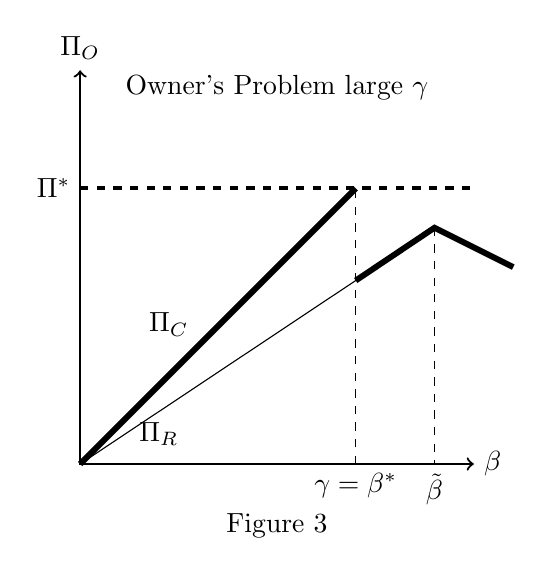
\begin{tikzpicture}[scale=0.5]
  \draw[thick,<->] (0,10) node[above]{$\Pi_{O}$}--(0,0)--(10,0) node[right]{$\beta$};
  \node [left] at (0,7) {$\Pi^{*}$};

\node [below] at (9,0) {$\tilde{\beta}$};
\node [below] at (7,0) {$\gamma = \beta^{*}$};

\node [above] at (5,9){Owner's Problem large $\gamma$};
%\node [above] at (5,10){};

\draw[line width=.75mm](0,0)--(7,7);
\draw[line width=.75mm](7,4.66)--(9,6)--(11,5);
\draw (0,0)--(7,4.66);

\node [above left] at (3,3){$\Pi_C$};
\node [below] at (2,1.3){$\Pi_R$};

\draw[dashed](9,6)--(9,0);
\draw[dashed](7,0)--(7,7);
\draw[dashed, line width=.5mm](0,7)--(10,7);

\node[below] at (5,-1){Figure 3};
  
\end{tikzpicture}
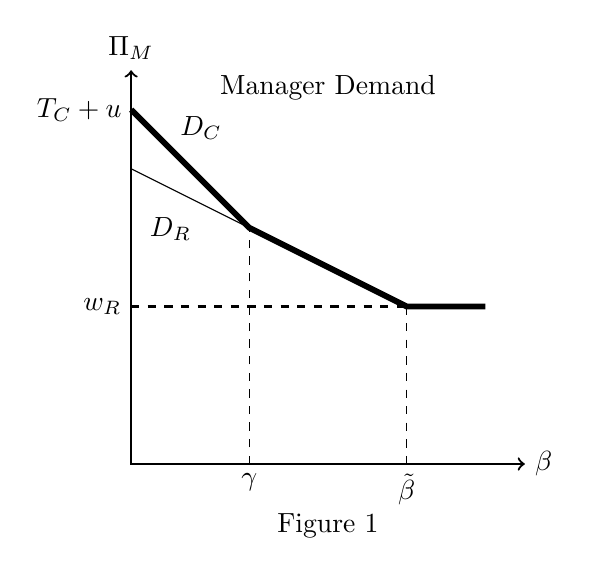
\begin{tikzpicture}[scale=0.5]

\draw[thick,<->] (0,10) node[above]{$\Pi_{M}$}--(0,0)--(10,0) node[right]{$\beta$};

\node [left] at (0,9) {$T_C + u$};
\node [left] at (0,4){ $w_R$};

\node [below] at (7,0) {$\tilde{\beta}$};
\node [below] at (3,0) {$\gamma$};
\node [above right] at (1,8){$D_C$};
\node [above] at (5,9){Manager Demand};

\draw[line width=.75mm](0,9)--(3,6)--(7,4)--(9,4);
\draw (0,7.5)--(3,6);
\node [below] at (1,6.5){$D_R$};

\draw[dashed](7,4)--(7,0);
\draw[dashed](3,0)--(3,6);
\draw[dashed, line width=.5mm](0,4)--(9,4);

\node[below] at (5,-1){Figure 1};

\end{tikzpicture}

\end{figure}










\end{document}
